%
% Documento: Fundamentação Teorica
%

%\vspace{3cm}%Espaçamento entre linhas

\chapter{\textbf{FUNDAMENTAÇÃO TEÓRICA}}\label{chap:fundTeorica}

A agropecuária familiar ocupou sempre um papel de destaque no Produto Interno Bruto (PIB) do Brasil. Segundo \citeonline{gui07} no período de análise (entre 1995 e 2005) o segmento familiar do agronegócio brasileiro respondeu por cerca de 10\% do PIB brasileiro, no qual 30\% é a parcela ocupada pelo próprio agronegócio no seu sentido mais amplo. No Rio Grande do Sul (RS), onde a pesquisa foi realizada, "a maior parte dos estabelecimentos agropecuários do RS enquadra-se nos critérios definidores da agricultura familiar" \cite{fee15}.

Para \citeonline{agroinf96}, para que se ocorra o progresso das agroindústrias familiares, é necessário que se supere dois fatores. O primeiro momento é fundamental que a sociedade entenda a importância e as vantagens da produção familiar, depois é preciso intensificar a qualidade e a produtividade nas mesmas. Ainda em \citeonline{agroinf96}, nessa fase a informática poderá ajudar, seja em agilizar processos ou facilitar a tomada de decisões.

Para melhor compreensão da maneira como o sistema foi desenvolvido, se faz necessário abordar os principais trabalhos relacionados, que de alguma forma contribuíram para algum atributo ou método do presente trabalho, também se faz importante conhecer as tecnologias utilizadas.

\section{TRABALHOS RELACIONADOS}


Durante o levantamento de dados foram buscadas plataformas que trabalham de forma semelhante ao presente sistema, como por exemplo o BovControl, o JetBov e o A3Pecuária, que serão apresentadas a seguir.

\subsection{\textbf{BovControl}}

BovControl é uma ferramenta de coleta e análise de dados provenientes da pecuária para melhorar a performance da produção de carne, leite ou genética \cite{bovcontrol10}.

É disponibilizado em forma de aplicativo e possui um plano gratuito, no qual é possível gerir um rebanho e faz os seguintes manejos nos animais: saída, lote, exame de toque, controle reprodutivo, idade da cria, idade do desmame, medicamento, origem, pesagem, perímetro escrotal, leite, teste diagnóstico, tipo de entrada, vacina, vermifugação. Também é possível visualizar seus dados em um dashboard\footnote{"Dashboards são painéis que mostram métricas e indicadores importantes para alcançar objetivos e metas traçadas de forma visual, facilitando a compreensão das informações geradas." \cite{nascimento17}.} na internet.

Possui uma parte de relatórios com apenas 2 gráficos, um do total de animais e do tipo de produção do animal (como leite, engorda e genética), e outro do total de animais e do gênero (macho ou fêmea).

Possui 3 planos profissionais que variam de R\$ 22,99 a R\$ 32,99 por mês. Estes planos incluem gestor financeiro, gestor de tarefas, multiusuários, relatórios personalizados, importação de animais por planilha e estoque de maquinário.

A Figura 1, é uma imagem mostrando a página inicial do sistema BovControl versão web com uma linha do tempo das ações efetuadas no aplicativo, a quantidades de animais por finalidade, e a quantidade de animais por gênero.

\begin{figure}[H]
	\begin{center}
		\caption{Dashboard do BovControl}
		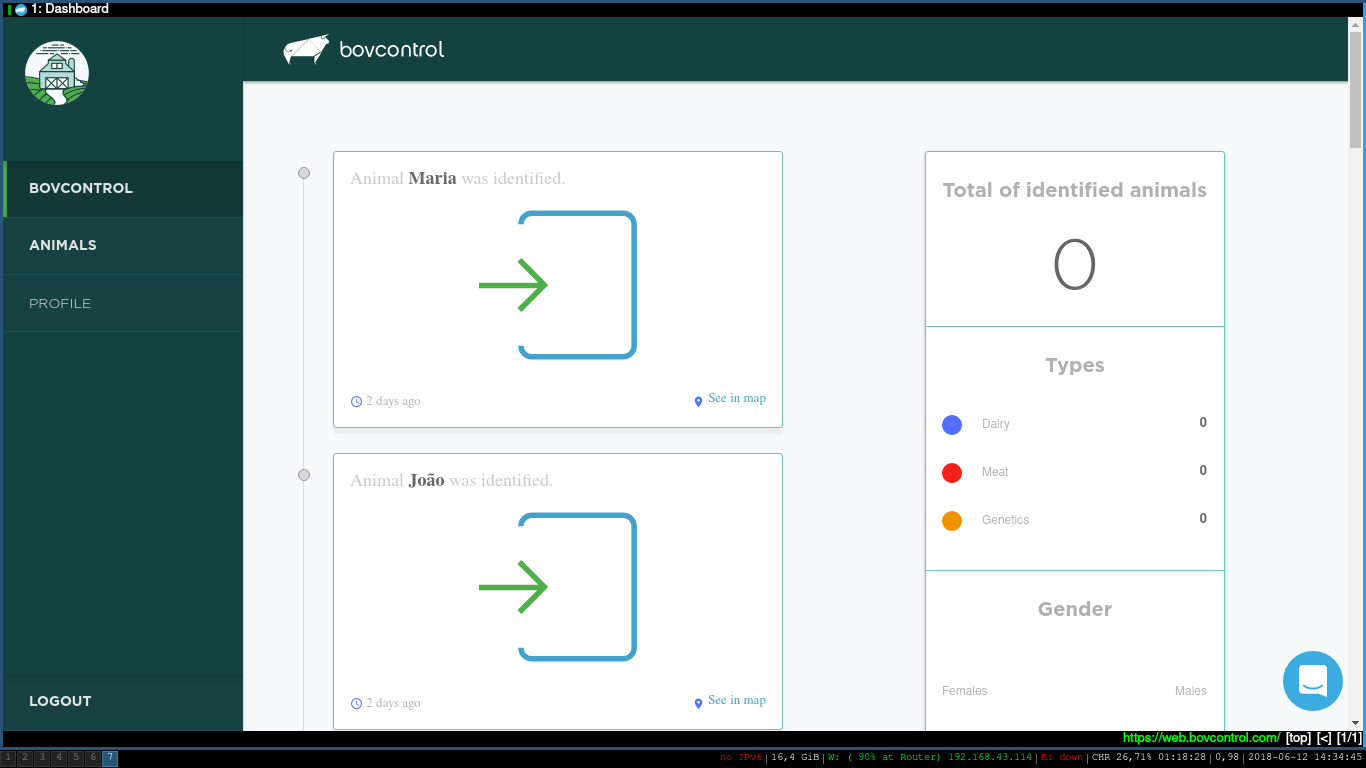
\includegraphics[width=\textwidth]{../img/bovcontrol.png}

		Fonte: Captura de tela do sistema BovControl.
	\end{center}
\end{figure}


%\begin{figure}[!h]
%\begin{center}
%\caption{BovControl versão mobile - Página inicial}
%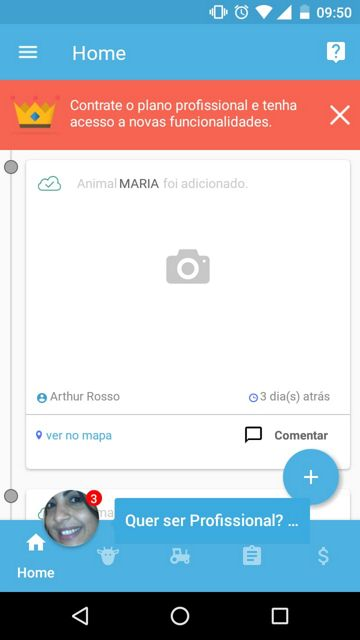
\includegraphics[width=6in]{img/bovcontrolapp1.jpg}

% % %\floatfoot{Fonte: Autoria própria.}
%\end{center}
%\end{figure}

%\begin{figure}[!h]
%\begin{center}
%\caption{BovControl versão mobile - Opções de ações}
%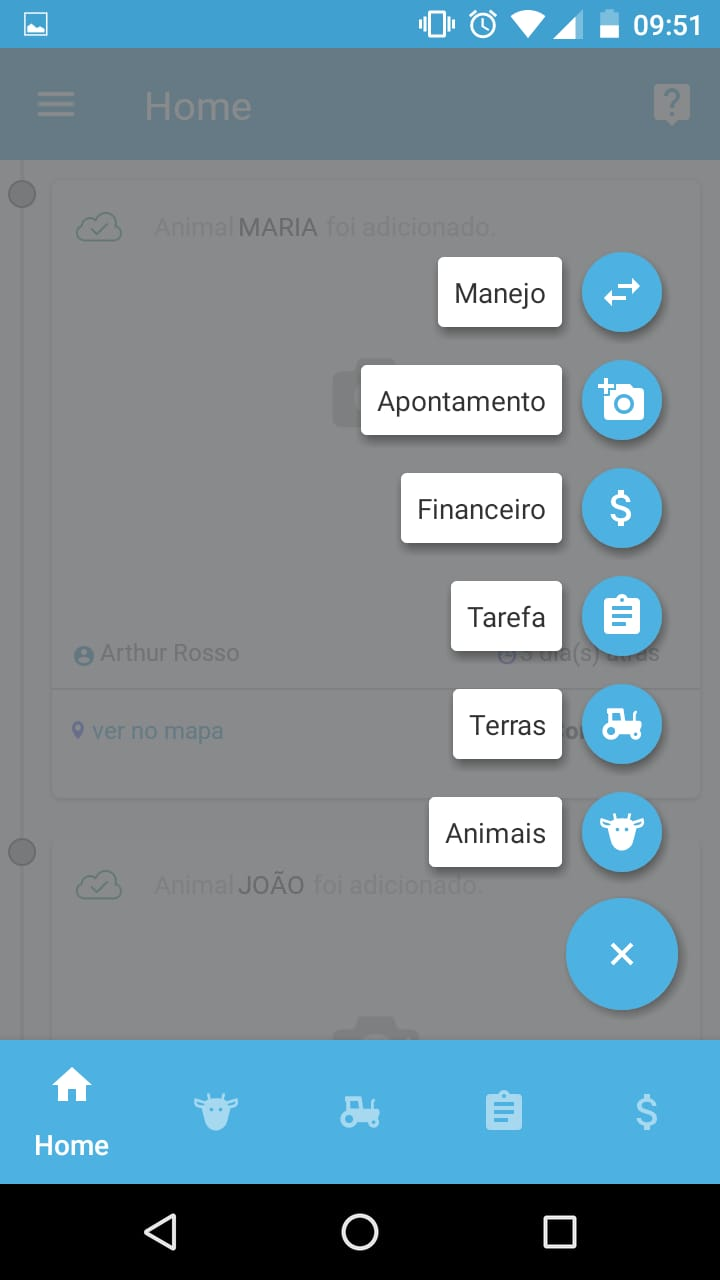
\includegraphics[width=6in]{img/bovcontrolapp2.jpeg}

% %\floatfoot{Fonte: Autoria própria.}
%\end{center}
%\end{figure}


\subsection{\textbf{JetBov}}

Segundo \citeonline{jetbov16}, esse é um sistema que tem como objetivo a gestão da fazenda, da cria até a terminação, a pasto, no semi-confinamento ou confinamento, com um controle de custos com o propósito de aumento da rentabilidade.

Não possui versão gratuita, porém há uma versão de testes disponível por 21 dias, após isso é necessário realizar um orçamento individual.

O sistema apresenta 2 versões, uma Web e outra Mobile, sendo a segunda mais reduzida contendo apenas uma página com animais e um botão contendo as opções de manejo como adicionar um novo animal e sua identificação, registros sanitários como vacinações, medicações, exames, vermifugações, etc, adicionar a morte de um animal, o desmame, o parto e pesagem.

A versão Web é mais completa contendo um painel de dados da fazenda, com gráficos de animais por sexo, animais por lote, peso por lote e algumas informações como número total de animais da fazenda, peso total da fazenda.

A Figura 2 apresenta uma captura de tela da página a página inicial do sistema JetBov versão Web após o Login, nela é apresentada uma série de informações sobre a propriedade, como o total de animais, o peso total de todos os animais o ganho médio de peso por dia quanto vale a arroba do boi gordo no dia. Mais abaixo dessas informações são mostrados gráficos de pizza que indicam as fatias de animais por gênero, lote e peso total por lote. No menu lateral são apresentadas todas as opções que podem ser feitas no sistema.

\begin{figure}[H]
	\begin{center}
		\caption{Página inicial da versão web do JetBov}
		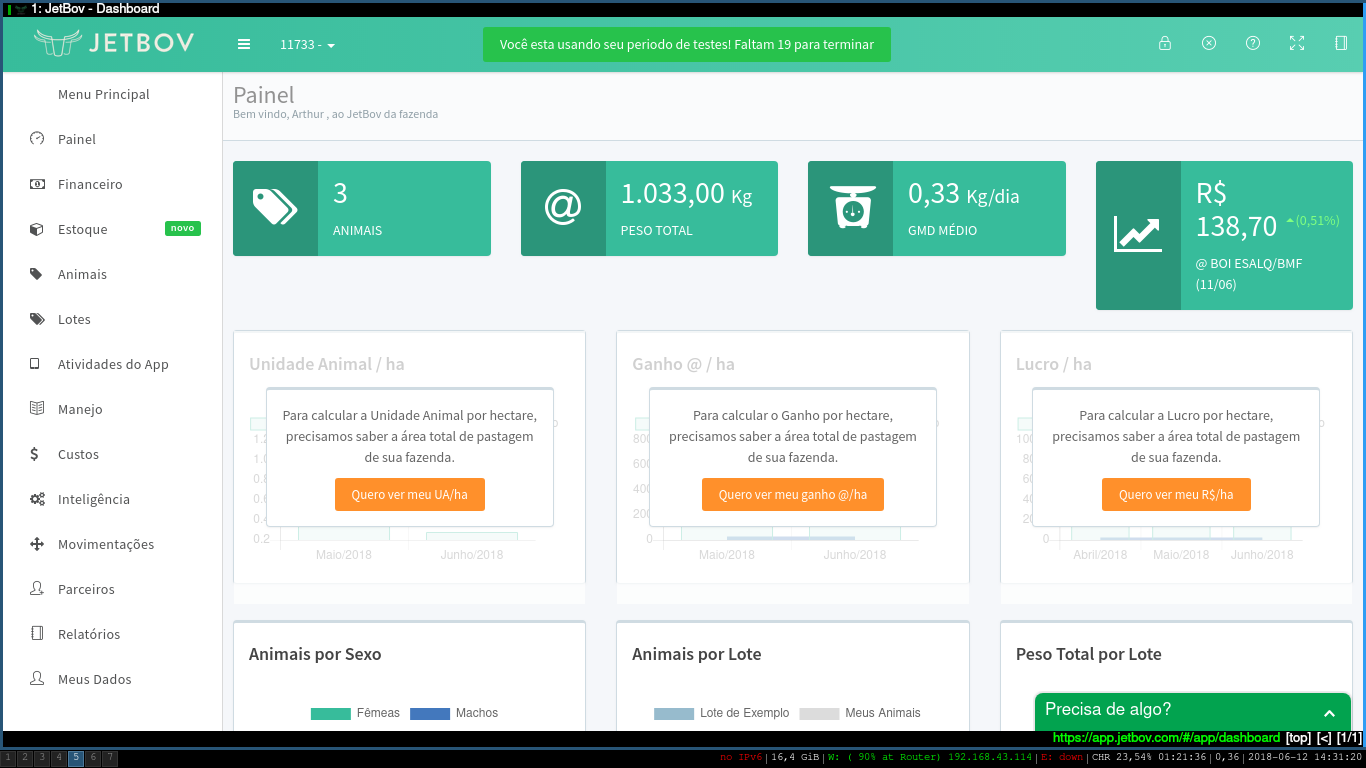
\includegraphics[width=\textwidth]{../img/jetbov.png}

		Fonte: Captura de tela do sistema JetBov.
	\end{center}
\end{figure}

%\begin{figure}[!h]
%\begin{center}
%\caption{Jetbov versão mobile - Página inicial}
%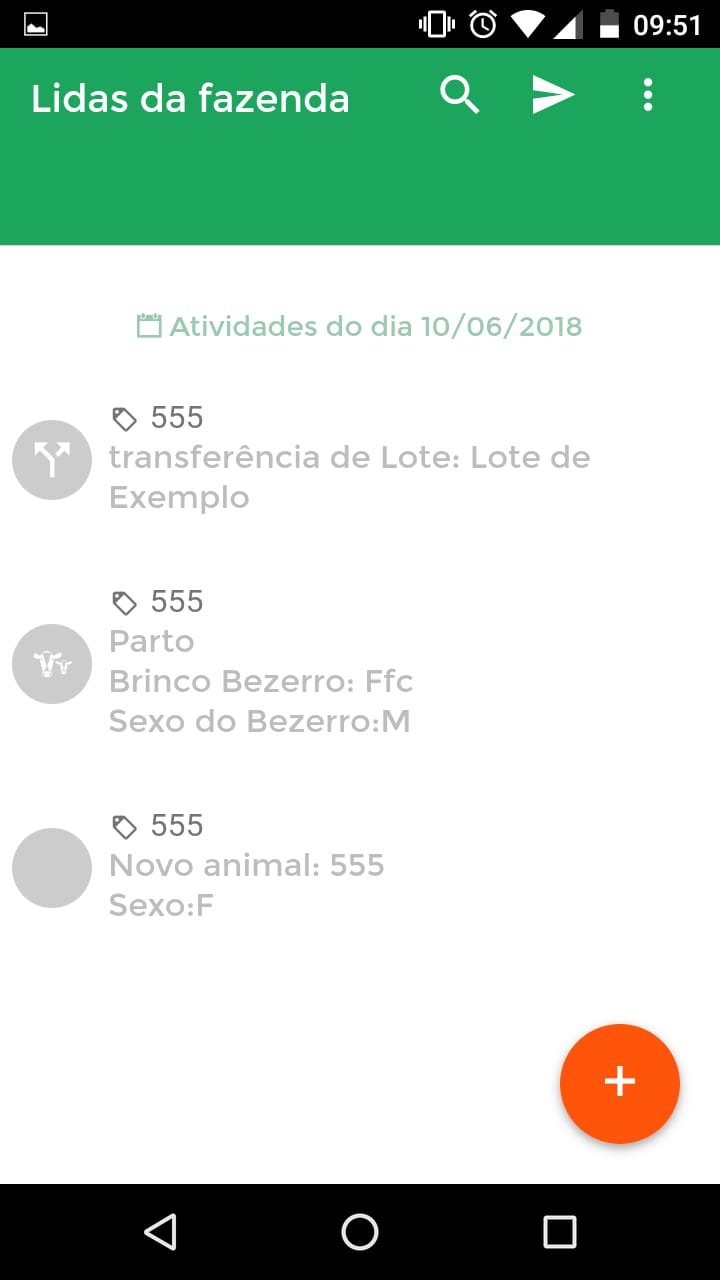
\includegraphics[width=6in]{img/jetbovapp1.jpeg}

% %\floatfoot{Fonte: Autoria própria.}
%\end{center}
%\end{figure}

%\begin{figure}[!h]
%\begin{center}
%\caption{JetBov versão mobile - Opções de ações}
%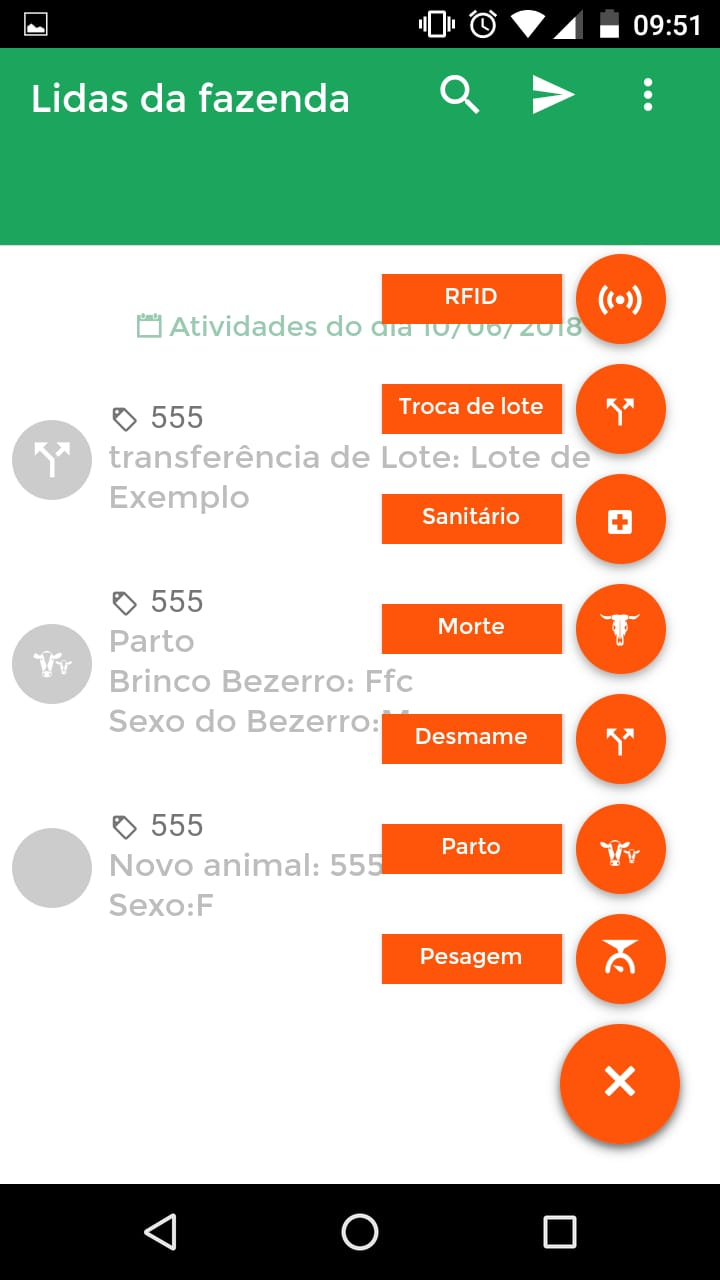
\includegraphics[width=6in]{img/jetbovapp2.jpeg}

% %\floatfoot{Fonte: Autoria própria.}
%\end{center}
%\end{figure}

\subsection{\textbf{A3Pecuária}}

A3Pecuária é um software para gestão de animais com controle de reprodução, pesagens, vacinas, exames, controle financeiro, estoque, compra e venda. Segundo o site do fabricante: "fornecemos importantes informações de análise de seu rebanho de maneira simples e com uma interface muito fácil de aprender, permitindo gerir seu investimento de forma a aumentar a lucratividade"  \cite{a3pecuaria16}.

Segundo \citeonline{a3pecuaria16}, são 3 tipos de planos, que variam de R\$ 29,90 a R\$ 69,90 por mês, e que gerenciam 500 animais ativos e 1 Fazenda até 3000 animais ativos e fazendas ilimitadas. Não possui versão gratuita, mas uma versão de testes por 30 dias.

Apresenta duas versões, uma web e outra mobile. A mobile, por ser mais reduzida, contém apenas a lista de animais da fazenda, o inventário, uma opção de bastão eletrônico e links para a versão web.

A versão Web, por ser mais completa, apresenta uma série de possibilidades de manejos como novo lote, novo animal, nova despesa, nova receita e uma série de análise de dados com relatórios da propriedade.

A figura 3, uma imagem mostrando a página inicial do sistema A3Pecuária versão Web. Nos cartões coloridos estão as informações de total de animais identificados, não identificados, fêmeas cobertas, fêmeas prenhas. Também há um módulo com mensagens de um representante da empresa e gráficos de avisos, referentes ao cadastro de novas categorias, animais que se encontram no fim da fase de lactação, número de medicações, lembretes e novos animais.


\begin{figure}[H]
	\begin{center}
		\caption{Página inicial da versão web do A3Pecuária}
		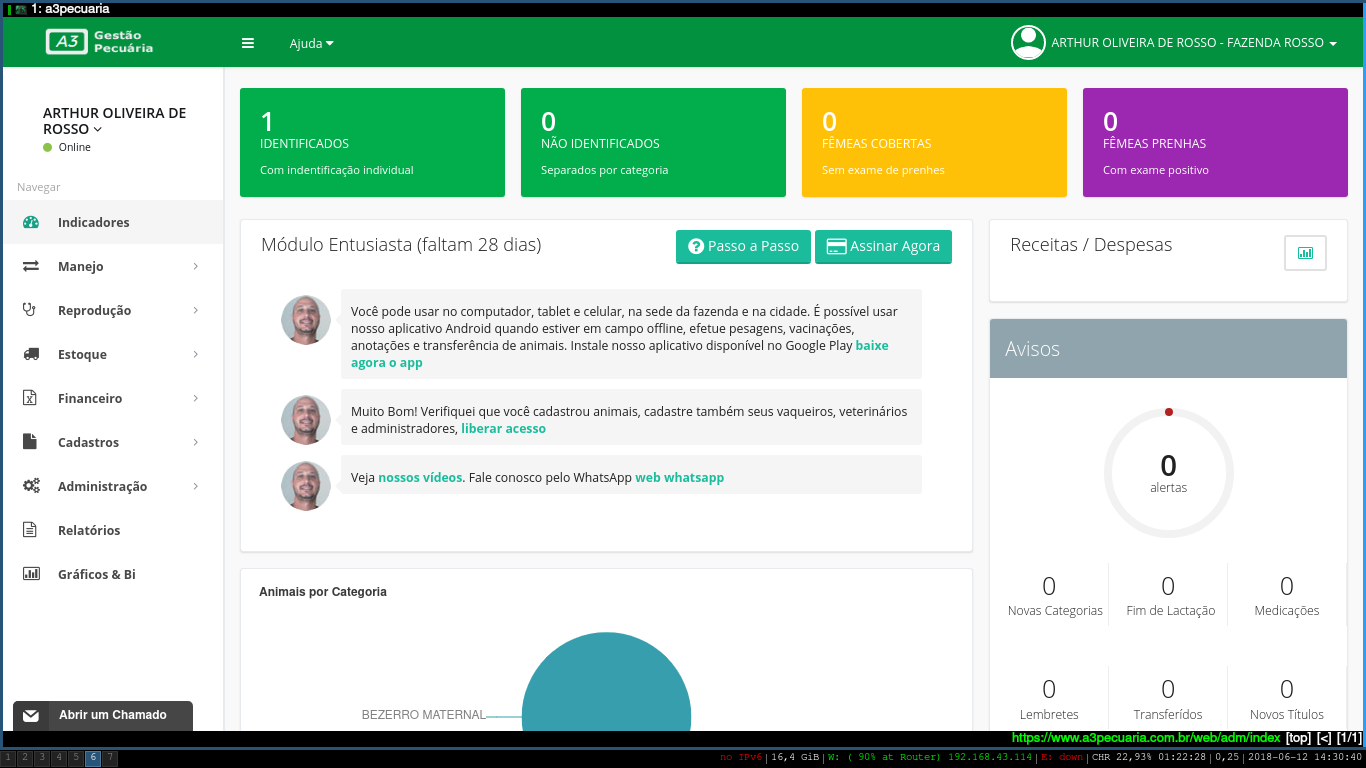
\includegraphics[width=\textwidth]{../img/a3pecuaria.png}

		Fonte: Captura de tela do sistema A3Pecuária.
	\end{center}
\end{figure}

%\begin{figure}[!h]
%\begin{center}
%\caption{A3Pecuária versão mobile - Página inicial}
%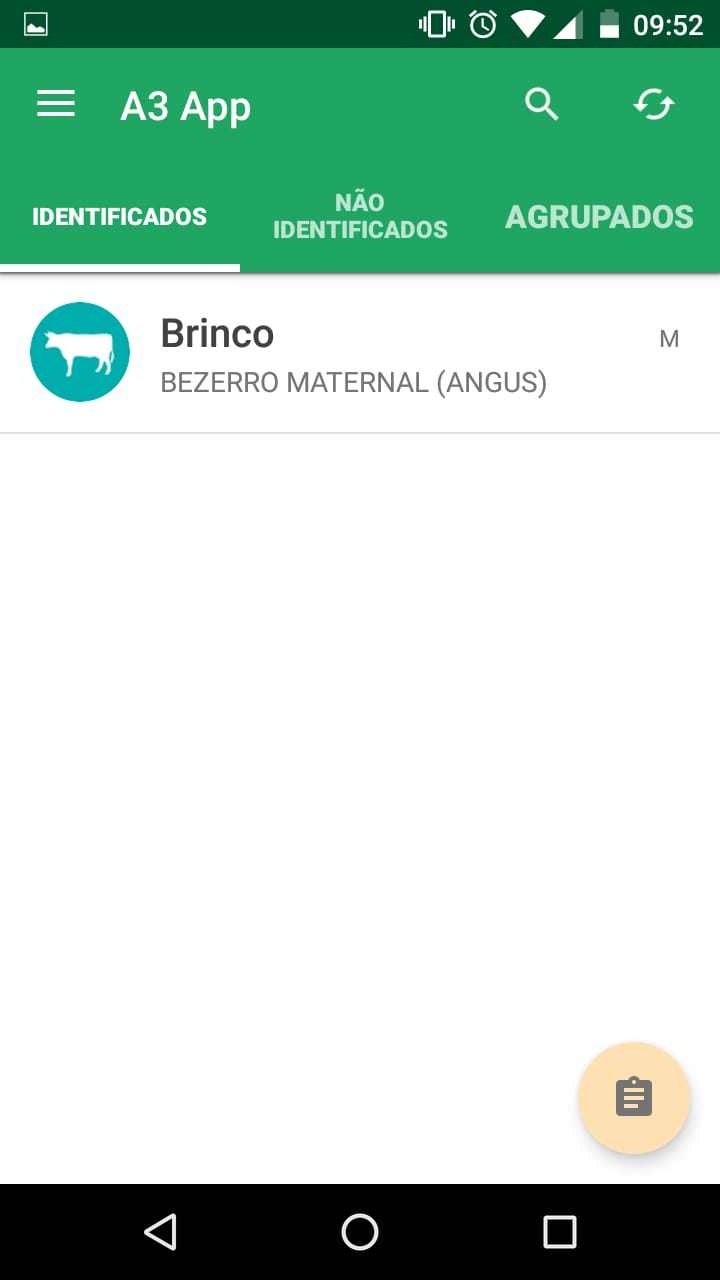
\includegraphics[width=6in]{img/a3pecuariaapp1.jpeg}

% %\floatfoot{Fonte: Autoria própria.}
%\end{center}
%\end{figure}

%\begin{figure}[!h]
%\begin{center}
%\caption{A3Pecuária versão mobile - Opções de ações}
%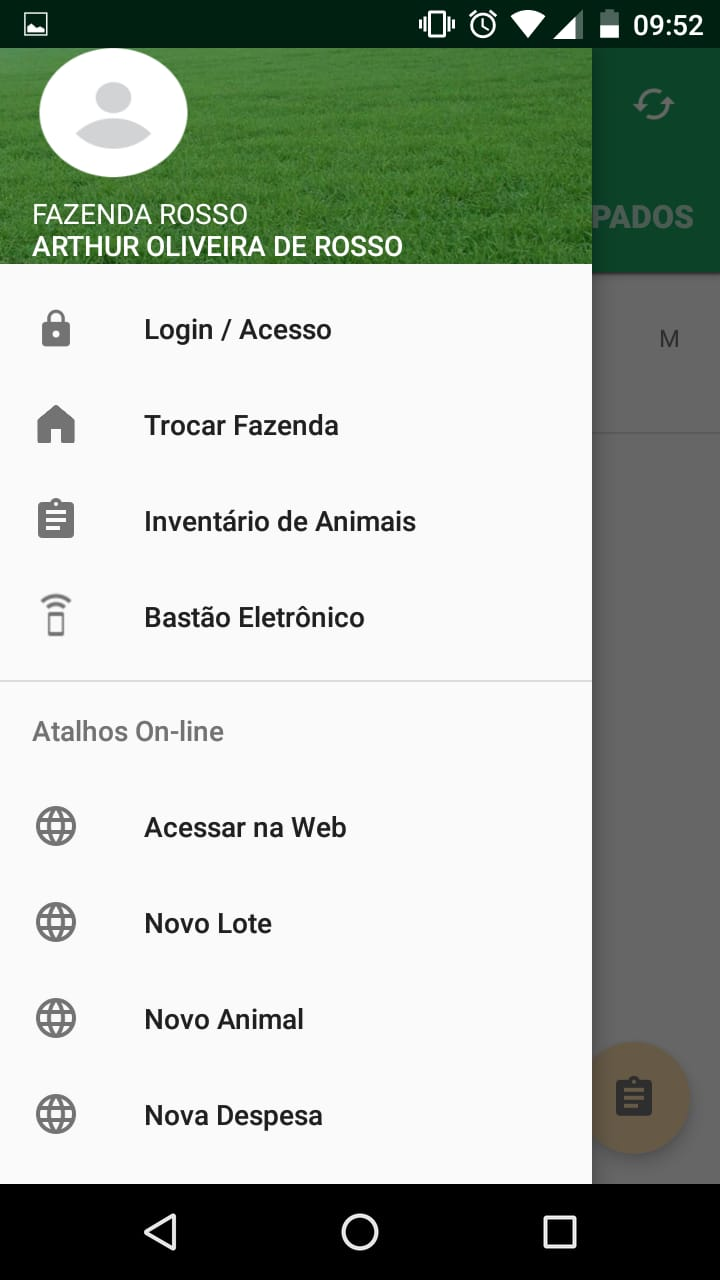
\includegraphics[width=6in]{img/a3pecuariaapp2.jpeg}

% %\floatfoot{Fonte: Autoria própria.}
%\end{center}
%\end{figure}

\subsection{\textbf{Análise Comparativa dos Trabalhos Relacionados}}

A partir da análise feita nas plataformas, pode-se chegar na seguinte conclusão: todas tem seu modo de operação semelhante, como criar, deletar, ler e editar as informações de um animal, e as opções de tratamento de gado (aqui chamado de manejo). As opções de estoque, que no proposto sistema é trabalhado só com medicações e a visualização de relatórios são trabalhados de maneira parecida em todos os sistemas também. Dessa maneira o sistema tem por objetivo trabalhar com estas mesmas operações, de maneira mais transparente, acessível e sem custos.


\begin{table}[H]
	\begin{center}
		\caption{Tabela da análise dos trabalhos relacionados}
		\begin{tabular}{ | p{8cm} |  c | c | c | c |}
			\hline
			Funcionalidade & BovControl & JetBov & A3Pecuária & GoBov \\ \hline
			Gerenciamento de animais de uma propriedade & Sim & Sim & Sim & Sim \\  \hline
			Gerenciamento do estoque de medicamentos  & Não & Não & Sim & Sim  \\ \hline
			Gerenciamento de medicações de animais & Sim & Sim & Sim & Sim  \\ \hline
			Visualização de relatórios gerais da propriedade & Sim & Sim & Sim & Sim  \\ \hline
			Visualização de relatórios individuais de cada animal & Não & Não & Não & Sim  \\ \hline
			Possibilidade de exportar para excel & Não & Não & Não & Sim  \\ \hline
			Versão gratuita & Sim & Não & Não & Sim  \\
			\hline
		\end{tabular}
		Fonte: Autoria própria.
	\end{center}
\end{table}


\section{TECNOLOGIAS UTILIZADAS}\label{tec}

Esta seção tratará as tecnologias que foram utilizadas na produção do presente trabalho. Bem como os motivos de suas escolhas.

A linguagem utilizada no \textit{backend}\footnote{"Sistema responsável pela regra de negócios, webservices e APIs de uma aplicação."\cite{lamim14}} é Go, uma linguagem de programação de código aberto que facilita a criação de software simples, bastante adequada para pequenos e médios projetos.

Sua utilização se justifica pela facilidade de realizar os CRUD (\textit{Create, Read, Update e Delete}, são as quatro operações básicas utilizadas em dados ou em bases de dados relacionais); baixa abstração o que deixa o ritmo de produção de código rápido uma vez que não é necessário pesquisar o que cada método é responsável; métodos precisos para as necessidades do problema.

\begin{lstlisting}
// Hello World em Go!
package main

import "fmt"

func main() {
	fmt.Println("Hello, World!")
}
\end{lstlisting}

Foram utilizados dois Sistemas Gerenciadores de Banco de Dados (SGBD) no projeto, um local na máquina do pesquisador, o MariaDB, trata-se de um SGBD de código aberto bastante conhecido, é um \textit{fork}\footnote{Segundo \citeonline{sil15} forks são ramificações de projetos já existentes.} do MySQL, e outro para o servidor remoto, para que funcione no Heroku\footnote{Servidor escolhido como o ambiente final de produção. Disponível em:
<https://www.heroku.com/>}, o PostgreSQL, o "PostgreSQL é um sistema de gerenciamento de banco de dados objeto-relacional (SGBDOR) baseado no POSTGRES Versão 4.2 desenvolvido pelo Departamento de Ciência da Computação da Universidade da Califórnia em Berkeley."  \cite{postgres07}.

Para a construção do \textit{frontend}\footnote{"Interface de interação com o usuário."\cite{lamim14}} foi utilizada a linguagem de marcação HTML que providencia a estrutura da página, para os estilos CSS. JavaScript, que é uma linguagem de programação que executa scripts no lado do cliente também foi utilizada. Também se utilizou o framework Materialize, como um facilitador da estilização das páginas HTML, assim foi possível deixa-las responsivas.

Como \textit{template engine} foi utilizado o Mustache, com ele é possível mostrar nas páginas do navegador o conteúdo do banco de dados. Pelo fato de não utilizar lógica, todas as regras de negócio ficam restritas a linguagem do servidor.

GORM é uma biblioteca Mapeamento Objeto Relacional (ORM) para Go, ele torna desnessessária a manipulação de código de Linguagem de Consulta Estruturada (SQL) diretamente, facilitando assim o trânsito entre diferentes SGBD. Ele também torna o projeto mais seguro, uma vez que o deixa imune a \textit{SQL Injection}.

Gorilla é um conjunto de pacotes para desenvolver em Go para web, entre elas as usadas foram o gorilla/mux que providencia um sofisticado acesso a rotas com váriaveis e \textit{middleware}. Outro pacote utilizado foi o gorilla/session para a manipulação das sessões, e utilizando as \textit{flashes}.
